% Options for packages loaded elsewhere
\PassOptionsToPackage{unicode}{hyperref}
\PassOptionsToPackage{hyphens}{url}
\PassOptionsToPackage{dvipsnames,svgnames,x11names}{xcolor}
%
\documentclass[
]{article}

\usepackage{amsmath,amssymb}
\usepackage{iftex}
\ifPDFTeX
  \usepackage[T1]{fontenc}
  \usepackage[utf8]{inputenc}
  \usepackage{textcomp} % provide euro and other symbols
\else % if luatex or xetex
  \usepackage{unicode-math}
  \defaultfontfeatures{Scale=MatchLowercase}
  \defaultfontfeatures[\rmfamily]{Ligatures=TeX,Scale=1}
\fi
\usepackage{lmodern}
\ifPDFTeX\else  
    % xetex/luatex font selection
\fi
% Use upquote if available, for straight quotes in verbatim environments
\IfFileExists{upquote.sty}{\usepackage{upquote}}{}
\IfFileExists{microtype.sty}{% use microtype if available
  \usepackage[]{microtype}
  \UseMicrotypeSet[protrusion]{basicmath} % disable protrusion for tt fonts
}{}
\makeatletter
\@ifundefined{KOMAClassName}{% if non-KOMA class
  \IfFileExists{parskip.sty}{%
    \usepackage{parskip}
  }{% else
    \setlength{\parindent}{0pt}
    \setlength{\parskip}{6pt plus 2pt minus 1pt}}
}{% if KOMA class
  \KOMAoptions{parskip=half}}
\makeatother
\usepackage{xcolor}
\setlength{\emergencystretch}{3em} % prevent overfull lines
\setcounter{secnumdepth}{-\maxdimen} % remove section numbering
% Make \paragraph and \subparagraph free-standing
\ifx\paragraph\undefined\else
  \let\oldparagraph\paragraph
  \renewcommand{\paragraph}[1]{\oldparagraph{#1}\mbox{}}
\fi
\ifx\subparagraph\undefined\else
  \let\oldsubparagraph\subparagraph
  \renewcommand{\subparagraph}[1]{\oldsubparagraph{#1}\mbox{}}
\fi


\providecommand{\tightlist}{%
  \setlength{\itemsep}{0pt}\setlength{\parskip}{0pt}}\usepackage{longtable,booktabs,array}
\usepackage{calc} % for calculating minipage widths
% Correct order of tables after \paragraph or \subparagraph
\usepackage{etoolbox}
\makeatletter
\patchcmd\longtable{\par}{\if@noskipsec\mbox{}\fi\par}{}{}
\makeatother
% Allow footnotes in longtable head/foot
\IfFileExists{footnotehyper.sty}{\usepackage{footnotehyper}}{\usepackage{footnote}}
\makesavenoteenv{longtable}
\usepackage{graphicx}
\makeatletter
\def\maxwidth{\ifdim\Gin@nat@width>\linewidth\linewidth\else\Gin@nat@width\fi}
\def\maxheight{\ifdim\Gin@nat@height>\textheight\textheight\else\Gin@nat@height\fi}
\makeatother
% Scale images if necessary, so that they will not overflow the page
% margins by default, and it is still possible to overwrite the defaults
% using explicit options in \includegraphics[width, height, ...]{}
\setkeys{Gin}{width=\maxwidth,height=\maxheight,keepaspectratio}
% Set default figure placement to htbp
\makeatletter
\def\fps@figure{htbp}
\makeatother
\newlength{\cslhangindent}
\setlength{\cslhangindent}{1.5em}
\newlength{\csllabelwidth}
\setlength{\csllabelwidth}{3em}
\newlength{\cslentryspacingunit} % times entry-spacing
\setlength{\cslentryspacingunit}{\parskip}
\newenvironment{CSLReferences}[2] % #1 hanging-ident, #2 entry spacing
 {% don't indent paragraphs
  \setlength{\parindent}{0pt}
  % turn on hanging indent if param 1 is 1
  \ifodd #1
  \let\oldpar\par
  \def\par{\hangindent=\cslhangindent\oldpar}
  \fi
  % set entry spacing
  \setlength{\parskip}{#2\cslentryspacingunit}
 }%
 {}
\usepackage{calc}
\newcommand{\CSLBlock}[1]{#1\hfill\break}
\newcommand{\CSLLeftMargin}[1]{\parbox[t]{\csllabelwidth}{#1}}
\newcommand{\CSLRightInline}[1]{\parbox[t]{\linewidth - \csllabelwidth}{#1}\break}
\newcommand{\CSLIndent}[1]{\hspace{\cslhangindent}#1}

\usepackage{booktabs}
\usepackage{longtable}
\usepackage{array}
\usepackage{multirow}
\usepackage{wrapfig}
\usepackage{float}
\usepackage{colortbl}
\usepackage{pdflscape}
\usepackage{tabu}
\usepackage{threeparttable}
\usepackage{threeparttablex}
\usepackage[normalem]{ulem}
\usepackage{makecell}
\usepackage{xcolor}
\usepackage{mathtools}
\makeatletter
\makeatother
\makeatletter
\makeatother
\makeatletter
\@ifpackageloaded{caption}{}{\usepackage{caption}}
\AtBeginDocument{%
\ifdefined\contentsname
  \renewcommand*\contentsname{Table of contents}
\else
  \newcommand\contentsname{Table of contents}
\fi
\ifdefined\listfigurename
  \renewcommand*\listfigurename{List of Figures}
\else
  \newcommand\listfigurename{List of Figures}
\fi
\ifdefined\listtablename
  \renewcommand*\listtablename{List of Tables}
\else
  \newcommand\listtablename{List of Tables}
\fi
\ifdefined\figurename
  \renewcommand*\figurename{Figure}
\else
  \newcommand\figurename{Figure}
\fi
\ifdefined\tablename
  \renewcommand*\tablename{Table}
\else
  \newcommand\tablename{Table}
\fi
}
\@ifpackageloaded{float}{}{\usepackage{float}}
\floatstyle{ruled}
\@ifundefined{c@chapter}{\newfloat{codelisting}{h}{lop}}{\newfloat{codelisting}{h}{lop}[chapter]}
\floatname{codelisting}{Listing}
\newcommand*\listoflistings{\listof{codelisting}{List of Listings}}
\makeatother
\makeatletter
\@ifpackageloaded{caption}{}{\usepackage{caption}}
\@ifpackageloaded{subcaption}{}{\usepackage{subcaption}}
\makeatother
\makeatletter
\@ifpackageloaded{tcolorbox}{}{\usepackage[skins,breakable]{tcolorbox}}
\makeatother
\makeatletter
\@ifundefined{shadecolor}{\definecolor{shadecolor}{rgb}{.97, .97, .97}}
\makeatother
\makeatletter
\makeatother
\makeatletter
\@ifpackageloaded{sidenotes}{}{\usepackage{sidenotes}}
\@ifpackageloaded{marginnote}{}{\usepackage{marginnote}}
\makeatother
\makeatletter
\makeatother
\ifLuaTeX
  \usepackage{selnolig}  % disable illegal ligatures
\fi
\IfFileExists{bookmark.sty}{\usepackage{bookmark}}{\usepackage{hyperref}}
\IfFileExists{xurl.sty}{\usepackage{xurl}}{} % add URL line breaks if available
\urlstyle{same} % disable monospaced font for URLs
\hypersetup{
  pdftitle={The Implementation of China's Overseas NGO Law and the Operating Space for International Civil Society},
  pdfauthor={Meng Ye; Andrew Heiss},
  pdfkeywords={international NGOs, civil
society, authoritarianism, Chinese ONGO law},
  colorlinks=true,
  linkcolor={blue},
  filecolor={Maroon},
  citecolor={Blue},
  urlcolor={Blue},
  pdfcreator={LaTeX via pandoc}}

\title{The Implementation of China's Overseas NGO Law and the Operating
Space for International Civil Society}
\author{Meng Ye \and Andrew Heiss}
\date{2023-04-07}

\begin{document}
\maketitle
\begin{abstract}
China's 2017 Overseas NGO (ONGO) Law is part of a larger global trend of
legal restrictions on international NGOs (INGOs). However, the effects
of this global crackdown on INGOs have been difficult to measure since
there is often divergence between the formal de jure regulations and the
de facto implementation of these laws. Additionally, the severity and
consistency of the enforcement of these laws often depends on the type
of services provided by these organizations. In this paper, we measure
the effect of China's ONGO law on INGO operations in the five years
since the passage of the law. We test whether and how INGO operational
space under the ONGO law is influenced by organizations' issue areas. We
argue that the less contensious the issue areas INGOs work in the more
likely they are granted greater operational space, measured by thenumber
of provinces they are allowed to work in by the registration
documentation. China provides an excellent setting for testing the
``closing space'' and ``changing space'' theoretical understanding
because the 2017 ONGO law hypothetically regulates both claim-making and
service-providing NGOs, while the level of ambiguity of the law gives
ample room for arbitrary discretion and conflicting attitudes by
authorities. We test our argument by analyzing administrative data from
633 registered representative offices of INGOs registered in China
between 2017--2021 and test our hypothesis with multilevel Bayesian
models. Our results speak to the broader literature on closing civic
space and provide an empirical illustration of the practical effect of
NGO restrictions on global civil society.
\end{abstract}
\ifdefined\Shaded\renewenvironment{Shaded}{\begin{tcolorbox}[breakable, boxrule=0pt, sharp corners, frame hidden, borderline west={3pt}{0pt}{shadecolor}, enhanced, interior hidden]}{\end{tcolorbox}}\fi

\hypertarget{introduction}{%
\section{Introduction}\label{introduction}}

In recent decades, there has been a global tend of ``closing space'' for
civil society across jurisdictions such as Russia, India and
Vietnam.{[}Dupuy and Prakash
(\protect\hyperlink{ref-DupuyPrakash:2020}{2020}); Chaudhry and Heiss
(\protect\hyperlink{ref-ChaudhryHeiss:2020}{2020});
(\protect\hyperlink{ref-Heiss2017}{\textbf{Heiss2017?}}); Sidel
(\protect\hyperlink{ref-Sidel:2023}{2023}); AtiaHerrold:2018{]}
(\emph{to update citation}). An ubiquitous manifestation of such trend
is rolling out restrictive laws that regulate international NGOs
(INGOs).(\protect\hyperlink{ref-DupuyPrakash:2020}{Dupuy and Prakash
2020}; \protect\hyperlink{ref-ChaudhryHeiss:2022a}{Chaudhry and Heiss
2022a}). China's promulgation of the Law of the People's Republic of
China on Administration of Activities of Overseas Nongovernmental
Organizations in the Mainland of China (the ``ONGO Law'') on April 28,
2016 was considered part of a recent global wave of legal restrictions
on INGOs. As an authoritarian jurisdiction with a growing nonprofit
sector, the Chinese model of implementing restrictive laws for INGOs has
great implications for scholarly understanding of the dynamics of how
such laws are used as policy tools to harness INGOs in practice. The
purpose of this study is to empirically examine how the ONGO Law has
impacted INGO's presence as well as the operational space after the law
took effect. By inquiring the \emph{de facto} implementation of the law
in addition to formal \emph{de jure} regulations, we intent to inquire
into a more comprehensive and data-based picture of the operational
space for INGOs. It will also test out the evolving theory of the
``closing space'' or ``changing space'' for INGOs hold true in a
representative empirical setting of the mainland China.

INGOs came to China after the Reform and Opening-up policy was adopted
by the authority and have been playing pivotal roles in providing
funding, organizational and program management skills, as well as
catalytic support for the emergence of China's domestic nonprofit sector
(\protect\hyperlink{ref-Yin:2009}{Yin 2009}). Before the promulgation of
the ONGO Law, the regulation of INGOs in China was obscure
{[}Shieh:2018; Spires:2022{]}. The only legal document relevant to INGOs
was a section of the Regulation on the Management of Foundations by the
State Council that specifies the registration of representative offices
(``ROs'') of foreign foundations with the Ministry of Civil Affairs, the
regulator of Chinese domestic NGOs. However, the actual application of
the regulation was very limited. Up until the ONGO Law took effect on
January 1, 2017, there were fewer than 30 foreign foundation ROs
registered at the Ministry of Civil Affairs according to the Regulation
on the Management of Foundations, while some Chinese officials estimated
in 2016 that there were roughly over 7000 ONGOs operating in China
(\protect\hyperlink{ref-YeHuang:2018}{Ye and Huang 2018}).

Many INGOs gained legal identity within mainland China using the vehicle
of foreign-funded companies {[}Sidel:2016{]}, though there were no clear
requirements for them to have a formal legal presence in
China(\protect\hyperlink{ref-Han:2011}{Han 2011}). They choose to have a
formal legal identity for the convenience such as signing labor
contracts directly with employees. However, the legal form of
foreign-funded company is not quite compatible with the nature of ONGOs.
Under the Chinese legal system, enterprises should be for-profit
entities and nonprofit organizations are required to choose other
stand-alone legal forms for them --- foundations, associations and
social service organizations (\protect\hyperlink{ref-Ye:2021}{Ye 2021}).
Thus, ONGOs obtaining legal identity in this way have to navigate
through a legal framework designed for the for-profit institutional
logic, e.g, focusing on project investors' right to investment return.

The legal framework governing ONGOs was overhauled by the Chinese ONGO
Law. The new law applies to all Overseas (including Hong Kong, Macau and
Taiwan) non-governmental organizations that conduct not-for-profit
activities in the fields of Economic Development, Education, Science,
Technology, Culture, Public Health, Sports, Environment Protection,
Poverty Alleviation, and Disaster Relief etc. (Article 3). In other
words, after the Overseas NGOs became effective, any nonprofit
activities conducted by those ONGOs that cannot successfully obtaining
proper legal authorization according to the law will be deemed illegal.
Specifically, the ONGO law stipulates two ways to lawfully conduct
nonprofit activities in China for ONGOs: registering ROs or filing
information for documentation of temporary activities with the Ministry
of Public Security (``MPS'') and Provincial-level Public Security
bureaus, which are the registering and regulatory authority for ONGOs
designated by the law. Registering an RO would be lawful identity
gaining channel for INGOs seeking for on-going presence in China while
temporary activities are suitable for INGOs that need to conduct one-off
programs that last no longer than one year.

This paper studies the the empirical data of the registration of ROs in
the years following the enactment of the ONGO Law to uncover the
association between INGO issue areas and the composition of successful
RO registration and the operational space granted. Registering RO under
the ONGO Law requiring the consent of a Chinese professional supervisory
unit (the ``PSU''), which are governmental or quasi-governmental
overseeing the INGO's issue area to co-supervise the INGOs with Public
Security bureaus. And it turns out that obtaining the consent of a PSU
to apply for registration became a key challenge for ONGOs, because
potential PSUs do not have a legal obligation to assume such a demanding
role (\protect\hyperlink{ref-Jia:2017}{Jia 2017};
\protect\hyperlink{ref-Shieh:2018}{Shieh 2018};
\protect\hyperlink{ref-YeHuang:2018}{Ye and Huang 2018}). Therefore, the
composition of the successfully registered RO inform us whether ROs
working on different issue areas have varied level of difficulty in
obtaining legal status. Moreover, We measure the later with a proxy of
the number of provinces that the ROs are authorized to operate.
Specifically, the registration document of an RO would specify the field
of work and mission for the RO and list the range of provinces that the
RO is authorized to conduct nonprofit activities in (Article 18). Some
ROs are authorized to operate across mainland China, which is 32
provincial administrative regions in total, but there are also many that
are authorized to operate in one to multiple provinces but not all. We
use the number of provinces that ROs are authorized to work in as a
proxy to measure the operational space for INGOs in China based on the
empirical understanding that INGOs need to or hope to have the approval
to be able to carry out their programs in a geographical scope as larger
as possible. (\protect\hyperlink{ref-Li:2020}{Li 2020})

\hypertarget{literature-and-theoretical-background}{%
\section{Literature and Theoretical
Background}\label{literature-and-theoretical-background}}

\hypertarget{literature-on-closing-space-for-ingos}{%
\subsection{Literature on Closing Space for
INGOs}\label{literature-on-closing-space-for-ingos}}

Contentiousness, regime stability, other reasons (to add studies on this
construct globally)

\hypertarget{literature-on-differenciated-attitudes-towards-ingos-as-reveal-in-implementation}{%
\subsection{Literature on differenciated attitudes towards INGOs (as
reveal in
implementation)}\label{literature-on-differenciated-attitudes-towards-ingos-as-reveal-in-implementation}}

``We discuss the role of civil society organizations (CSOs) as agents of
democratization and note the emergence of dual, at times apparently
conflicting policy postures within authoritarian regimes (restriction
and repression for some CSOs vs.~financial support and opportunities for
collaboration for others).''
(\protect\hyperlink{ref-ToeplerZimmerFrohlich:2020}{Toepler et al.
2020})

Also, (\protect\hyperlink{ref-Plantan2022}{\textbf{Plantan2022?}}) finds
``that I find'' evidence of selective implementation that reveals which
groups are seen as threatening or beneficial.''

\emph{de jure} vs.~\emph{de facto} difference ``represents a
bureaucratic form of repression''
(\protect\hyperlink{ref-ChaudhryHeiss:2022}{Chaudhry and Heiss 2022b})

The promulgation of China's ONGO Law has been discussed by scholars
mostly as a part of a global trend of restricting and cracking down
International NGOs
(\protect\hyperlink{ref-ChaudhryHeiss2022}{\textbf{ChaudhryHeiss2022?}};
\protect\hyperlink{ref-Carothers:2016}{Carothers 2016}). Studies on the
law has been focused on discussing the historical and political impetus
of passing the law (Shieh, 2018) or analyzing the regulatory regimes it
that has established and potential implications for INGOs operating in
China {[}Feng (\protect\hyperlink{ref-Feng:2017}{2017});Teets and Hsu
(\protect\hyperlink{ref-TeetsHsu:2016}{2016})). However, little work has
been done to examine the actual implementation situation of this law,
and how the dynamics of ONGOs' operations and projects have been
affected by the law after successfully gaining legal registration and
documentation. A couple of studies
(\protect\hyperlink{ref-Jia2017}{\textbf{Jia2017?}};
\protect\hyperlink{ref-YeHuang:2018}{Ye and Huang 2018})) conducted
reflections on the first year's implementation of China's ONGO Law,
including the initial phase of drafting and refining implementing
regulations and promotion, as well as training sessions conducted by
Public Security Bureaus in different locations. However, a more
up-to-date and comprehensive understanding of the effects of the ONGO
law is still lacking.

This paper aims to fill these gaps by empirically examining how the
``closing space'' hypothesis applies to China in the years after the
ONGO Law took effect. China provides an excellent setting for testing
these theories because China's promulgation of restrictive INGO law as
an authoritarian jurisdiction fits the observed global trends in recent
years, thus can serve as an representative case to deepen scholarly
understanding around these themes. Also, the level of ambiguity of the
legal framework gives ample room for arbitrary discretion and
conflicting attitudes by authorities, enabling us to analyze rules in
form (\emph{de jure}) as well as rules in use (\emph{de facto}).

Based on extant literature and theoretical understanding, we hypothesize
that the operation space INGOs are granted is associated with the level
of contentious their missions, i.e., the issue areas they work in. Since
the level of contentious is also manifested by the level of difficulty
they face while seeking lawful registration. We also hypothesize that
large operational space of INGOs is negatively associated the time
elapsed since the law took effect when they successfully got registered.

The follow section is structured as follow. In the data and methods
section, we first report the data cleaning and coding process and
measurements used in our empirical analysis. Then we explain the
rationale for choosing ordered beta regression to fit our models. In the
Results section, we report and interpret both descriptive analysis and
regression analysis results. We conclude the paper by discussing the
implications of our findings with respective to more general scholarly
understanding of the closing space of international civil society.

\hypertarget{data-and-methods}{%
\section{Data and methods}\label{data-and-methods}}

\hypertarget{data}{%
\subsection{Data}\label{data}}

The data used in this paper was collected from INGOs' public
registration documents disclosed by MPS's Overseas NGO Office on the
online service platform for INGOs. We also use ChinaFile's China ONGO
data for complementary purpose, we merge in the English organization
name in ChinaFile for the sake of transparency of our analysis to
broader communities. The data we collected spans from January 1, 2017,
when the law took effect, to December 31, 2021, with data for 633 ROs in
total. The filing document of ROs disclose the name, the registration
date, the registration authority (which public security bureau regulates
it), the PSU, the address and issue area or purposes of the RO and the
specific provinces they can work in. We code the variables we use in the
empirical analysis from the registration information. Most of the coding
and data cleaning work is objective data wrangling process, such as
parsing out the province each RO is in from the address, or calculating
the total number provinces approved in the registration document.
Meanwhile, the coding of issue areas are conducted by the authors based
on the areas set out Article 3 (specified above) and clustering of the
issue areas of the actually registered ROs. (to cross-validate among
authors).

\hypertarget{measurement}{%
\subsection{Measurement}\label{measurement}}

\hypertarget{dependent-variables}{%
\subsubsection{Dependent Variables}\label{dependent-variables}}

Our dependent variable is ``geo\_scope\_num'', the count of the total
number of provinces each RO is authorized to operate in. We derived this
variable from the specific list of authorized provinces as recorded in
the RO's registration documentation. As discussed above, we use this
measurement as a proxy for operational space for INGOs, because any
geographical constraints on the RO impacts on the flexibility of the
INGO operations. For example, in circumstances where emergency like the
COVID 19 pandemic hits, it would be extremely hard for INGOs to plan
beforehand which areas would need their service. Thus, we assume INGOs
that are not set up with any locally-bound purposes would need to or
hope to (if there is not yet such needs) be able to operate in as
broader geographical scope as possible.

\hypertarget{independent-variables}{%
\subsubsection{Independent Variables}\label{independent-variables}}

Our first independent variable is ``work\_field\_code1'', the issue area
we code from mission statement specified in the RO's registration
documentation. Given there is certain level of subjectivity in the
coding process, the coding of issue areas are cross-checked between the
researchers (to do). The coding rules for overlapping issue areas can be
found in the Appendix (to add). We decided to have 9 issue areas groups
based on list of lawful fields of work specified by the Article 3 of the
ONGO Law and how actual issue areas cluster for registered ROs.

Below is the list of issue areas INGOs' registered ROs are coded into.

\begin{itemize}
\tightlist
\item
  \textbf{Economy and trade}
\item
  \textbf{Environment} (including animal protection)
\item
  \textbf{Education} (including youth development)
\item
  \textbf{Charity and humanitarian} poverty alleviation, disaster
  relief, etc., including rural development
\item
  \textbf{Science and technology}
\item
  \textbf{Industry association}
\item
  \textbf{Health}, public health and health care system support
  (professional training)
\item
  \textbf{Arts and Culture} including sports and international culture
  exchange
\item
  \textbf{General}, usually grant-making organizations, Or working on
  general international communication, including among governments, or
  working on multiple fields not overlapping
\end{itemize}

Our second variable is ``time\_elapsed''. This variable is derived the
time difference between ROs' registration date and January 1, 2017 when
the law took effect. The longer the time elapsed since registration
should be achieved by INGOs, it indicates that it took longer time for
them to seek the content of both the PSU and Public Security Bureaus to
be their supervisions or regulators and grant them legal identity.

\hypertarget{control-variables}{%
\subsubsection{Control Variables}\label{control-variables}}

Our first control variable is ``local\_connet''. It is a dichotomous
variable indicating whether operating locally is built into the RO's
mission. There are cases where the aim or mission of the INGO attached
to a locality, either having a county or city name in their RO name or
purposes, or the INGO are actually set up by people in China and they
registered the RO to communicate between the ``hometown'' and the INGO
set up abroad. So we include this variable in our model to how having
local connection is associated with the operational space of ROs as well
as how the contentious level associates with operation space when we
account for this factor.

We also cluster our 633 RO cases by the province where they are
registered in our hierarchical Bayesian modeling. Thus, we account for
any variance caused by the socioeconomic and institutional differences
in various provinces of China. And the level province is the apporoiate
level to cluster because all the ROs are registered at the provincial
public security bureaus.

\hypertarget{regression-model}{%
\subsection{Regression Model}\label{regression-model}}

Our data provides us with rich descriptive detail of the types of INGOs
allowed to register in China following the advent of the ONGO law, and
we explore patterns in this data below. In addition to presenting
descriptive summary statistics, we create a multilevel Bayesian
regression model to examine the complex effects that issue area, local
connections, and registration timing have on organizational flexibility.
This approach allows us to hold specific variables constant and generate
predictions for hypothetical new, not-yet-registered INGOs, providing us
with stronger empirical implications. Additionally, Bayesian modeling
allows us to calculate the posterior distribution of our different
estimands. Rather than report a single value for the proportion of
registered INGOs worked on specific issues, we can estimate posterior
credible intervals that represent the probability that the true
proportion falls within a specific range. We report posterior medians
and 95\% credible intervals throughout our analysis. Importantly, these
intervals do not behave like more traditional frequentist confidence
intervals. Instead, they can be interpreted as the probability that a
reported estimate falls within the range, given the data and modeling
choices.

\begin{figure}

{\centering 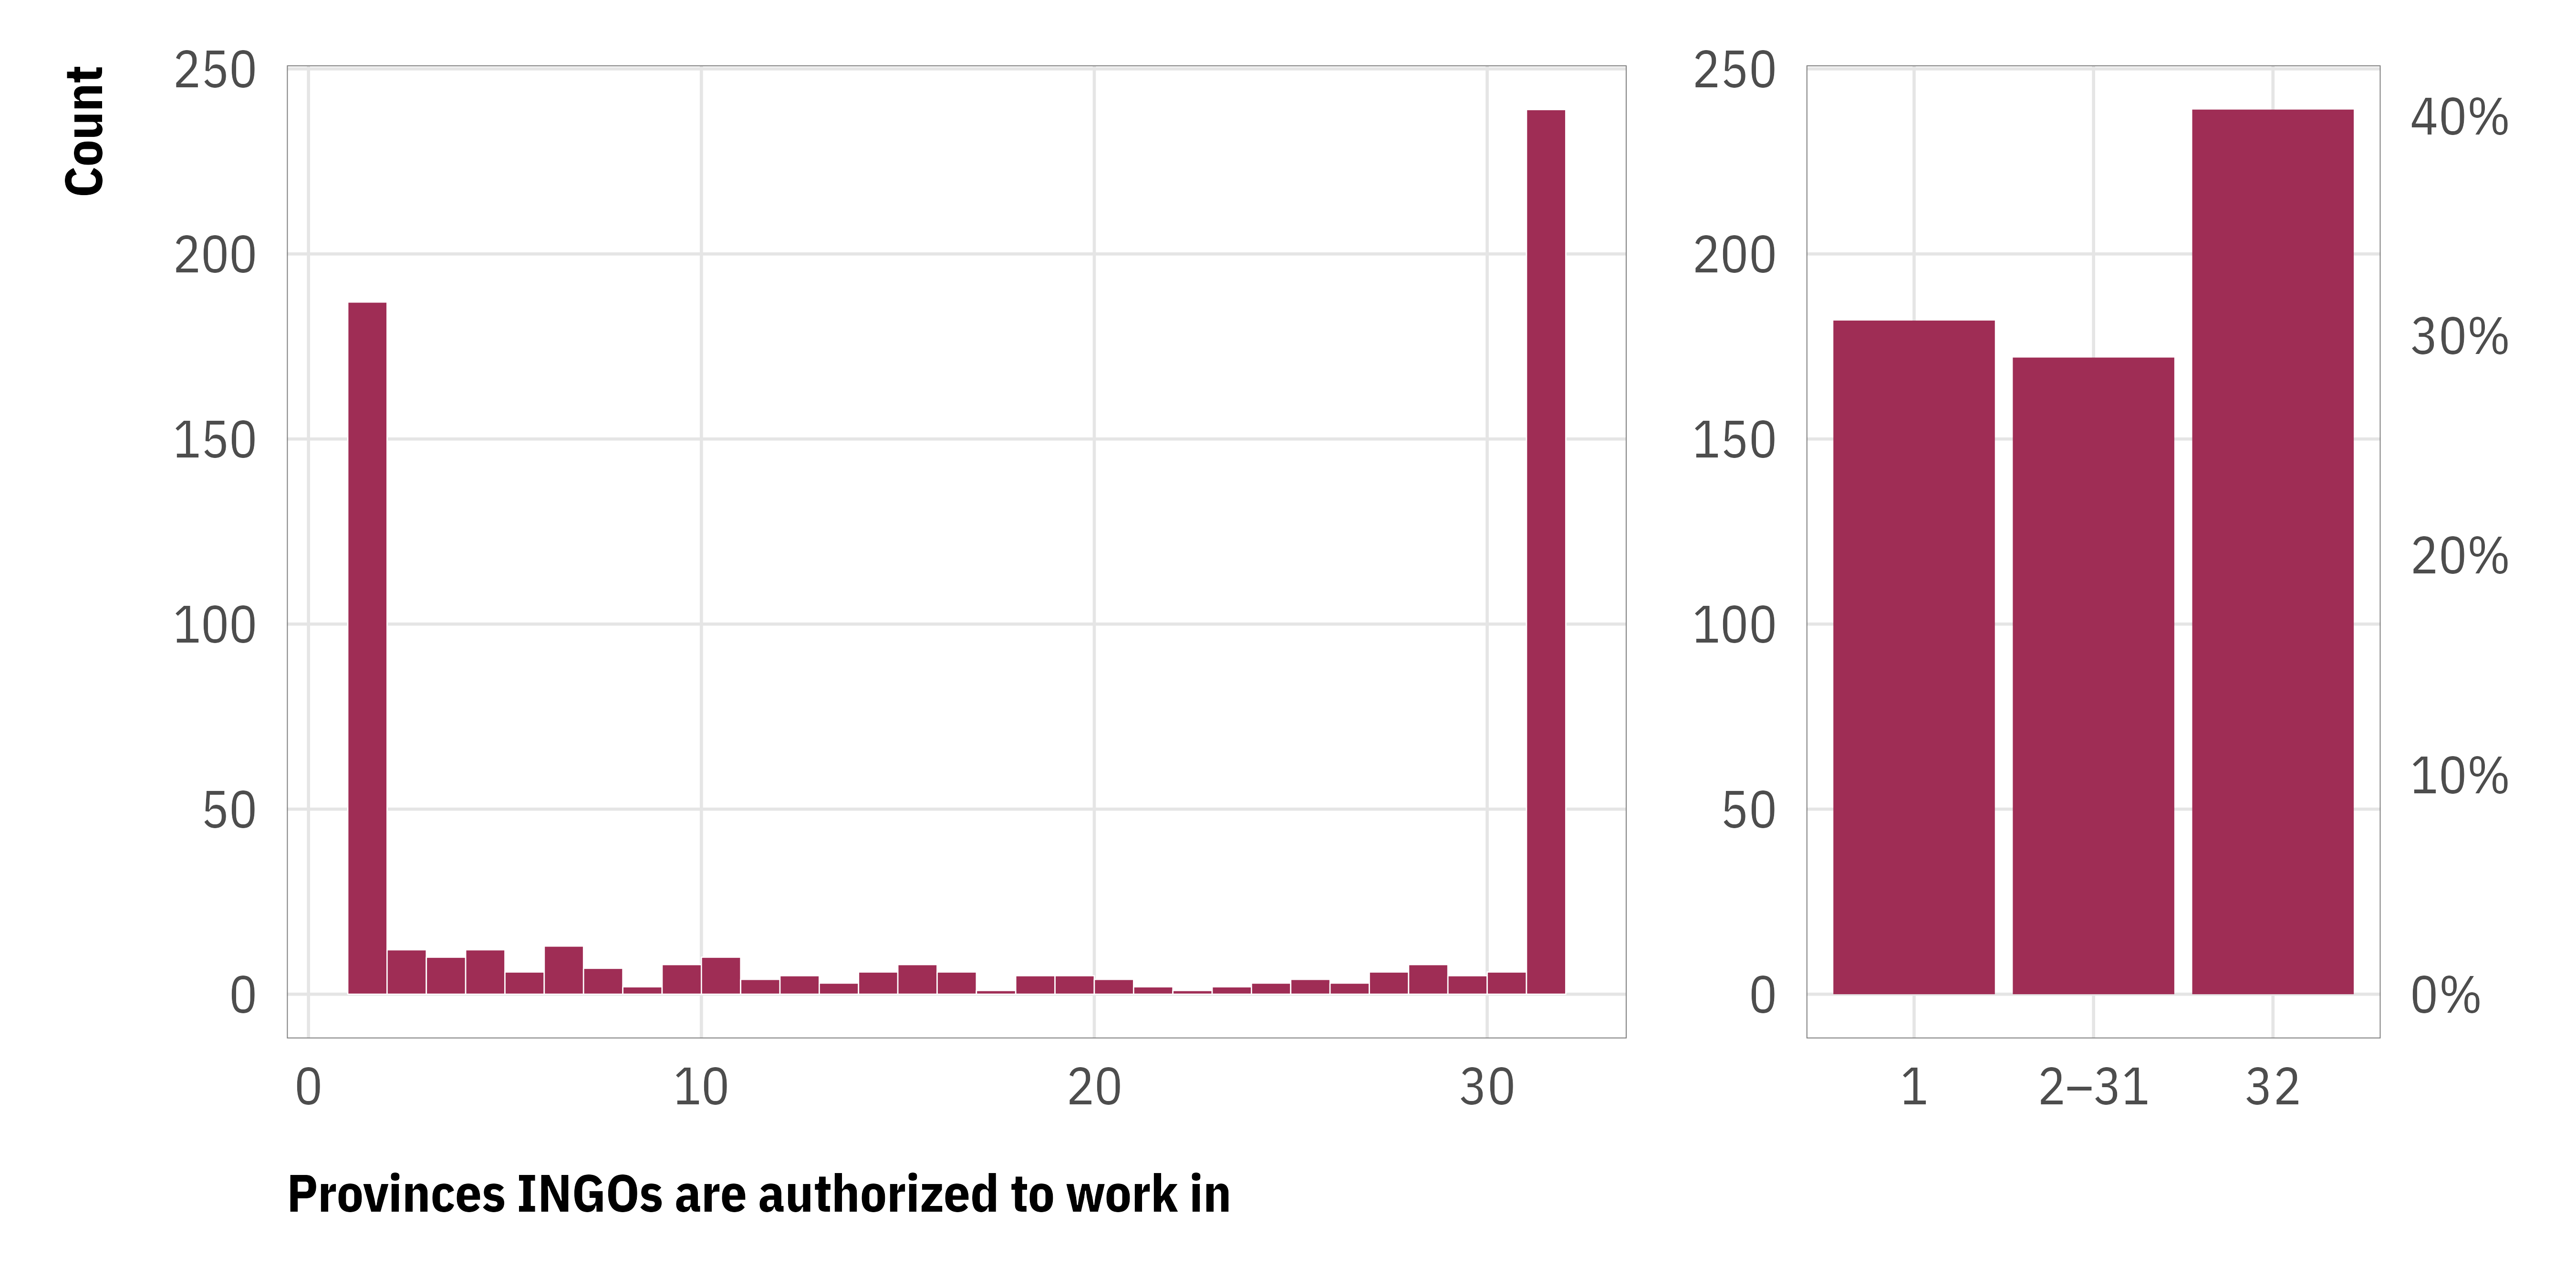
\includegraphics[width=0.8\textwidth,height=\textheight]{manuscript_files/figure-pdf/fig-province-count-collapsed-1.pdf}

}

\caption{\label{fig-province-count-collapsed}Count of the number of
provinces each INGO is authorized to operate in. The left panel shows
the full distribution of INGOs registered in 2--31 provinces; the right
panel collapses these in-between counts to a single category.}

\end{figure}

Modeling the count of provinces each INGO is authorized to operate in
presents a unique statistical challenge. As seen in
Figure~\ref{fig-province-count-collapsed}, roughly 30\% of INGOs are
registered in only one province, 40\% are registered nationwide, while
the remaining 30\% are registered in 2--31 provinces. Our main variable
of interest is thus a mix of continuous outcomes (i.e.~a range of
provinces) bounded between two discrete outcomes (i.e.~one province and
all provinces). Standard modeling approaches like ordinary least squares
regression (OLS) cannot accurately capture the unique features of the
data and will generate predictions that fall outside allowable bounds
(i.e.~negative counts of provinces or more than 32 provinces). If we
transform the count of provinces to a percentage, Beta regression would
work well, as it is naturally limited outcomes within a 0--1 range.
However, Beta regression cannot handle values that are exactly 0 or 1,
making it inappropriate for our data with its inflated counts at 0 (1)
and 100\% (32). To account for values at the bounds, we rely on ordered
Beta regression (\protect\hyperlink{ref-Kubinec:2022}{Kubinec 2022}),
and extension of zero-and-one-inflated Beta regression that allows us to
simultaneously model the continuous range of provinces (2--31) and the
discrete outcomes (1 province and 32 provinces) without relying on
percentages. We can thus explore the dynamics of each of our independent
variables of interest in multiple ways---we can see (1) how each
variable predicts that an organizations works in one province,
nationwide, or somewhere in between, and (2) how each variable predicts
the overall expected count of provinces.

Equation~\ref{eq-ordbeta} provides a formal definition of our modeling
choices. Since we are primarily interested in how an INGO's issue area,
its local connections, and the timing of its registration after January
2017, we include these as explanatory variables. We also include
province-specific random offsets for each intercept to account for
between-region differences in how INGOs are regulated. We use weakly
informative priors for all model parameters.

\begin{figure*}

\begin{equation}\protect\hypertarget{eq-ordbeta}{}{
\begin{aligned}
\text{Count of provinces}\ \sim&\ \operatorname{Ordered\ Beta}(\mu_{i_j}, \phi_y, k_{0_y}, k_{1_y}) & \text{Registered provinces for INGO $i$ in province $j$}\\[8pt]
\mu_{i_j} =&\ (\beta_0 + b_{0_j}) + \beta_1\ \text{Issue area}\ + & \text{Average outcome}\\
&\ \beta_2\ \text{Local connections}\ + \\
&\ \beta_3\ \text{Years since law took effect} \\
b_{0_j} =&\ \mathcal{N}(0, \sigma_0) & \text{Random province offsets} \\[8pt]
\beta_0\ \sim&\ \operatorname{Student\,t}(\nu = 3, \mu = 0, \sigma = 2.5) & \text{Prior for global intercept} \\
\beta_{1..3}\ \sim&\ \mathcal{N}(0, 5) & \text{Prior for global coefficients} \\
\sigma_0\ \sim&\ \operatorname{Student\,t}(3, 0, 2.5) & \text{Prior for between-province variability} \\
\phi_y\ \sim&\ \operatorname{Exponential}(1 / 100) & \text{Prior for within-province variability} \\
k_{0_y}, k_{1_y}\ \sim&\ \operatorname{Dirichlet}(1, 1, 1) & \text{Prior for 0–continuous and continuous–1 cutpoints} \\
\end{aligned}
}\label{eq-ordbeta}\end{equation}

\end{figure*}

\hypertarget{results}{%
\section{Results}\label{results}}

\hypertarget{descriptive-results}{%
\subsection{Descriptive Results}\label{descriptive-results}}

\hypertarget{regression-results}{%
\subsection{Regression Results}\label{regression-results}}

\hypertarget{issue-area}{%
\subsubsection{Issue area}\label{issue-area}}

\hypertarget{local-connections}{%
\subsubsection{Local connections}\label{local-connections}}

In our second empirical expectation, we posit that since INGOs that seek
out local connections and that are focused on more local China-specific
issues, those organizations should be registered in fewer provinces. The
results from our model confirm this expectation.

TODO 12ish expected provinces for INGOs with no local connections; 21ish
for INGOs with local connections

TODO We can take advantage of the continuous + discrete features of
ordered beta and see BLAH BLAH. After simulating 1,000 hypothetical new
INGOs, organizations without local connections are predicted to work
nationally in all provinces nearly 50\% of the time (ASDF-ASDF credible
interval), and are predicted to work in 2 or more provinces 35\% of the
time. These organizations with no local connections or local
programmatic focus are only predicted to work in a single province
15ish\% of the time. In contrast, INGOs \emph{with} local connections
are far more likely to only work in one province (35\%), or only work in
a handful of provinces. These locally-focused organizations are only
predicted to work nationally 25\% of the time.

TODO Graphs

\hypertarget{registration-timing}{%
\subsubsection{Registration timing}\label{registration-timing}}

\hypertarget{discussion}{%
\section{Discussion}\label{discussion}}

\hypertarget{references}{%
\section*{References}\label{references}}
\addcontentsline{toc}{section}{References}

\hypertarget{refs}{}
\begin{CSLReferences}{1}{0}
\leavevmode\vadjust pre{\hypertarget{ref-Carothers:2016}{}}%
Carothers, Thomas. 2016. {``Closing {Space} for {International
Democracy} and {Human Rights Support}.''} \emph{Journal of Human Rights
Practice} 8 (3): 358--77. \url{https://doi.org/10.1093/jhuman/huw012}.

\leavevmode\vadjust pre{\hypertarget{ref-ChaudhryHeiss:2020}{}}%
Chaudhry, Suparna, and Andrew Heiss. 2020. {``Closing {Space} and the
{Restructuring} of {Global Activism}: {Causes} and {Consequences} of the
{Global Crackdown} on {NGOs}.''}

\leavevmode\vadjust pre{\hypertarget{ref-ChaudhryHeiss:2022a}{}}%
---------. 2022a. {``Closing {Space} and the {Restructuring} of {Global
Activism Causes} and {Consequences} of the {Global Crackdown} on
{NGOs}.''} In \emph{Beyond the {Boomerang}: {From Transnational Advocacy
Networks} to {Transcalar Advocacy} in {International Politics}}, edited
by Christopher L. Pallas and Elizabeth A. Bloodgood, 23--35.
{Tuscaloosa, Alabama}: {University of Alabama Press}.

\leavevmode\vadjust pre{\hypertarget{ref-ChaudhryHeiss:2022}{}}%
---------. 2022b. {``{NGO} Repression as a Predictor of Worsening Human
Rights Abuses.''} \emph{Journal of Human Rights} 21 (2): 123--40.
\url{https://doi.org/10.1080/14754835.2022.2030205}.

\leavevmode\vadjust pre{\hypertarget{ref-DupuyPrakash:2020}{}}%
Dupuy, Kendra, and Aseem Prakash. 2020. {``Global {Backlash} Against
{Foreign Funding} to {Domestic Nongovernmental Organizations}.''} In
\emph{The {Nonprofit Sector}: {A Research Handbook}, {Third Edition28}.
{Global Backlash} Against {Foreign Funding} to {Domestic Nongovernmental
Organizations}}, 618--30. {Stanford University Press}.
\url{https://doi.org/10.1515/9781503611085-038}.

\leavevmode\vadjust pre{\hypertarget{ref-Feng:2017}{}}%
Feng, Chongyi. 2017. {``The {NGO} Law in {China} and Its Impact on
{Overseas} Funded {NGOs}.''} \emph{Cosmopolitan Civil Societies: An
Interdisciplinary Journal} 9 (3, 3): 95--105.
\url{https://doi.org/10.5130/ccs.v9i3.5601}.

\leavevmode\vadjust pre{\hypertarget{ref-Han:2011}{}}%
Han, Junkui. 2011. \emph{Overeseas NGO in China: Going Together with an
Opening-up China}. {Social Sciences Academic Press of China}.

\leavevmode\vadjust pre{\hypertarget{ref-Jia:2017}{}}%
Jia, Xijin. 2017. {``Analysis on the Effect of {China}'s Overseas {NGO}
Law Under the Differences in Legal Thinking.''} \emph{The China
Nonprofit Review} 9 (1): 23--43.

\leavevmode\vadjust pre{\hypertarget{ref-Kubinec:2022}{}}%
Kubinec, Robert. 2022. {``Ordered {Beta Regression}: {A Parsimonious},
{Well-Fitting Model} for {Continuous Data} with {Lower} and {Upper
Bounds}.''} \emph{Political Analysis}, 1--18.
\url{https://doi.org/10.1017/pan.2022.20}.

\leavevmode\vadjust pre{\hypertarget{ref-Li:2020}{}}%
Li, Shuoyan. 2020. {``Global {Civil Society Under} the {New INGO
Regulatory Law}: {A Comparative Case Study} on {Two INGOs} in
{China}.''} \emph{VOLUNTAS: International Journal of Voluntary and
Nonprofit Organizations} 31 (4): 751--61.
\url{https://doi.org/10.1007/s11266-019-00101-y}.

\leavevmode\vadjust pre{\hypertarget{ref-Shieh:2018}{}}%
Shieh, Shawn. 2018. {``The {Chinese State} and {Overseas NGOs}: {From
Regulatory Ambiguity} to the {Overseas NGO Law}.''} \emph{Nonprofit
Policy Forum} 9 (1). \url{https://doi.org/10.1515/npf-2017-0034}.

\leavevmode\vadjust pre{\hypertarget{ref-Sidel:2023}{}}%
Sidel, Mark. 2023. {``Vietnam's {Closing Legal Space} for {Civil
Society} --- {U}.{S}.-{Asia Law Institute}.''} {U.S.-Asia Law
Institute}. 2023.
\url{https://usali.org/usali-perspectives-blog/vietnams-closing-space-for-civil-society}.

\leavevmode\vadjust pre{\hypertarget{ref-TeetsHsu:2016}{}}%
Teets, Jessica, and Carolyn Hsu. 2016. {``Is {China} s {New Overseas NGO
Management Law Sounding} the {Death Knell} for {Civil Society}? {Maybe
Not}.''} \emph{The Asia-Pacific Journal}.

\leavevmode\vadjust pre{\hypertarget{ref-ToeplerZimmerFrohlich:2020}{}}%
Toepler, Stefan, Annette Zimmer, Christian Fröhlich, and Katharina
Obuch. 2020. {``The {Changing Space} for {NGOs}: {Civil Society} in
{Authoritarian} and {Hybrid Regimes}.''} \emph{VOLUNTAS: International
Journal of Voluntary and Nonprofit Organizations} 31 (4): 649--62.
\url{https://doi.org/10.1007/s11266-020-00240-7}.

\leavevmode\vadjust pre{\hypertarget{ref-Ye:2021}{}}%
Ye, Meng. 2021. {``Building an Enabling Legal Environment: Laws and
Policies on Social Enterprises in {China}.''} \emph{Journal of Asian
Public Policy} 14 (2): 182--99.
\url{https://doi.org/10.1080/17516234.2020.1824263}.

\leavevmode\vadjust pre{\hypertarget{ref-YeHuang:2018}{}}%
Ye, Meng, and Haoming Huang. 2018. {``Observations of the First Year
Implementation of the Law of Activities of Overseas NGOs in China.''} In
\emph{Annual Report on China's Philanthropy Development (2018)},
208--33. {Beijing}: {Social Sciences Academic Press of China}.

\leavevmode\vadjust pre{\hypertarget{ref-Yin:2009}{}}%
Yin, Deyong. 2009. {``China's {Attitude} Toward {Foreign NGOs}.''}
\emph{Washington University Global Studies Law Review} 8 (3): 521--44.
\url{https://heinonline.org/HOL/P?h=hein.journals/wasglo8\&i=529}.

\end{CSLReferences}



\end{document}
